\section{Conclusioni}
Il progetto è stato portato a termine entro i tempi previsti senza incontrare particolari problemi ed ogni membro del gruppo ha saputo gestire bene le tecnologie utilizzate per creare un sito internet efficiente dal punto di vista dei contenuti, dell'accessibilità e dell'usabilità. Sebbene sia stato usato HTML5 e CSS3 alcune funzioni di questi linguaggi, come ad esempio le canvas, non sono state utilizzate. Questa scelta è stata fatta perché l'utenza e le richieste del sito necessitano di poche funzionalità.\\
Infine sono stati eseguiti sul sito tutti i test di accessibilità riportati all'indirizzo \blue{\url{https://web.math.unipd.it/accessibility-dev/}}.

\begin{center}
    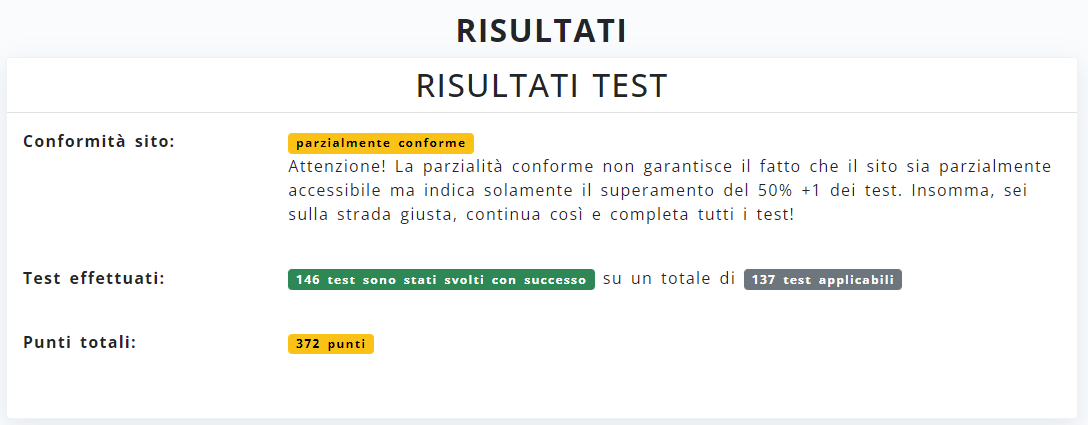
\includegraphics[scale=0.5]{images/test.png}
\end{center}